% ==============================================================================
% Pacote de Contribuição RQ1 (H-01 + H-02) — Pronto para integrar em paper/main.tex
% Não altera paper/main.tex diretamente para evitar conflitos de merge.
% Veja instruções linha a linha em paper/herik_contrib/INTEGRACAO_RQ1.md.
% Todos os números vêm de results/herik_e0/ e results/herik_h02/ (n = 595).
% ==============================================================================

% ------------------------------------------------------------------------------
% BLOCO 1: Substituir a frase da linha 32 no \begin{abstract} ... \end{abstract}
% (Original L32: "Diagnoses correlate with gold grades (QWK $0.49$) but are conservative.")
% ------------------------------------------------------------------------------
With the original prompt, diagnoses correlate with gold grades (QWK $0.49$) but are heavily conservative due to checklist artifacts (extra concepts, combining alternative references, and forced 3-gap lists); rubric calibration plus four cross-question anchor examples eliminates most of this bias (QWK $0.58$, $p_{\text{Holm}}{<}0.001$).

% ------------------------------------------------------------------------------
% BLOCO 2: Substituir a Subseção 5.1 (\subsection{Diagnosis (RQ1)}, L132-L140)
% Mantém Table~\ref{tab:confusion} original e referencia Table~\ref{tab:rq1_calib},
% Table~\ref{tab:rq1_confusion_v2} e Figure~\ref{fig:rq1_per_q} (no corpo ou apêndice).
% ------------------------------------------------------------------------------
\subsection{Diagnosis (RQ1)}
With the baseline prompt (\textbf{v0}), the estimated grade reaches QWK $=0.487$ (95\% question-clustered CI $[0.387, 0.586]$), Spearman $0.580$, MAE $0.703$, exact accuracy $42.9\%$ and binary ($\ge 2$) accuracy $67.7\%$ (range $0.179$--$0.784$ across questions). The diagnosis is strongly \emph{conservative} (bias $-0.380$; Table~\ref{tab:confusion}): $54.5\%$ of all predictions collapse onto grade~$1$, only $11$ of $145$ gold-$3$ answers are predicted as~$3$ ($46.2\%$ drop to $\le 1$), and $89$ of $150$ gold-$2$ answers drop to~$1$, while $43.3\%$ of gold-$0$ answers rise to $\ge 1$. Although not directly comparable, original human agreement ($r{=}0.58$, Pearson on a double-graded subset) suggests the baseline LLM approaches human rank ordering while suffering from severe calibration errors.

Error decomposition on the $595$ outputs reveals three prompt-induced mechanisms behind this bias. First, $53.7\%$ of severe under-gradings ($\text{gold}{=}3 \to \text{pred}\le 1$) and $51.7\%$ of $\text{gold}{=}2 \to 1$ cases have \emph{zero} conceptual errors listed; instead, the model adds extra rubric concepts in $61.5\%$ of items (mean $+1.06$) and penalizes omissions against the \emph{union} of alternative teacher references rather than checking equivalence to \emph{one} reference. Second, the model fills all three priority-gap slots in $97.8\%$ of items---including $92.4\%$ of gold-$3$ answers---and flags at least one ``conceptual error'' in $30.3\%$ of gold-$3$ answers. Third, leave-one-question-out (LOGO) post-hoc ordinal thresholding on internal diagnosis features raises QWK from $0.487$ to $0.575$ without new API calls, showing that most of the gap is scale miscalibration, whereas a few questions (\texttt{q36}, \texttt{q37}, \texttt{q42}, \texttt{q44}, \texttt{q48}) remain low ($<0.45$) due to semantic discrimination errors.

To fix these artifacts without post-hoc fitting, we evaluated two prompt-level calibrations on the same $595$ answers ($1{,}190$ OpenRouter calls, US\$$0.32$): \textbf{v1} removes extra-concept generation, states that teacher references are independent alternatives, allows $0$--$3$ gaps, distinguishes omissions from conceptual errors, and sharpens $0$--$3$ anchors; \textbf{v2} prepends four median-length anchor examples (grades $0$--$3$) drawn from a different question's disjoint holdout pool ($6{,}501$ unused PT-ASAG answers). Both gains are significant under question-clustered bootstrap with Holm correction ($p_{\text{Holm}}{=}0.0004$; Table~\ref{tab:rq1_calib}): \textbf{v1} reaches QWK $0.548$ ($+0.061$, $[0.033, 0.086]$) and \textbf{v2} reaches QWK $0.580$ ($+0.093$, $[0.062, 0.121]$), improving over \textbf{v0} on $14$ of $15$ questions (Figure~\ref{fig:rq1_per_q}), nearly eliminating bias ($-0.067$), cutting $\text{gold}{=}3 \to \le 1$ from $46.2\%$ to $20.0\%$, and slashing forced $3$-gap lists ($92.4\% \to 4.1\%$) and false conceptual errors ($30.3\% \to 2.8\%$) on gold-$3$ answers. Remaining side effects are mild over-scoring of gold-$0$ answers ($43.3\% \to 52.7\%$, explaining the single drop on \texttt{q40}), under-listing of broad curriculum tags in \texttt{q42}/\texttt{q49}, and gold-$3$ predictions still centering on~$2$ ($85/145$). Because pilot generation (E1/E3) was run with \textbf{v0}, Section~\ref{sec:setup} and~\S5.2--\S5.6 reflect the uncalibrated baseline; re-running downstream generation with \textbf{v2} is left for future work.

\begin{table}[t]
\centering\small
\begin{tabular}{lcccc}
\toprule
Gold $\backslash$ Predicted & 0 & 1 & 2 & 3 \\
\midrule
0 & 85 & 63 & 2 & 0 \\
1 & 16 & 107 & 27 & 0 \\
2 & 7 & 89 & 52 & 2 \\
3 & 2 & 65 & 67 & 11 \\
\bottomrule
\end{tabular}
\caption{Confusion matrix of baseline (\textbf{v0}) estimated vs.\ gold grade (E0, $n{=}595$).}
\label{tab:confusion}
\end{table}

\begin{table*}[t]
\centering\small
\begin{tabular}{lccccccc}
\toprule
Variant & QWK [95\% CI] & $\Delta$QWK & Spearman & MAE & Bias & 3-gap ($g{=}3$) & Err ($g{=}3$) \\
\midrule
Original prompt (v0) & 0.487 [0.387, 0.586] & -- & 0.580 & 0.703 & $-0.380$ & 92.4\% & 30.3\% \\
Calibrated rubric, zero-shot (v1) & 0.548 [0.450, 0.639] & $+0.061$* & 0.591 & 0.671 & $-0.166$ & 6.2\% & \textbf{2.8\%} \\
v1 + cross-question anchors (v2) & \textbf{0.580} [0.480, 0.678] & $+0.093$* & \textbf{0.609} & \textbf{0.635} & \textbf{$-0.067$} & \textbf{4.1\%} & \textbf{2.8\%} \\
\midrule
\emph{Post-hoc LOGO calibration (v0)} & \emph{0.575} & \emph{$+0.088$} & \emph{0.577} & \emph{0.711} & \emph{$+0.166$} & -- & -- \\
\bottomrule
\end{tabular}

\caption{Diagnosis calibration on PT-ASAG E0 ($n{=}595$; \texttt{gpt-4o-mini}, temp.\ $0$). $\Delta$QWK CIs use $5{,}000$ question-clustered bootstrap resamples; $^{*}$: Holm-adjusted $p{<}0.05$ across the two calibration contrasts vs.\ \textbf{v0}. \textit{3-gap} / \textit{Err ($g{=}3$)}: share of gold-$3$ answers receiving 3 forced gaps or $\ge 1$ conceptual error. Bottom row shows 15-fold LOGO post-hoc thresholding on \textbf{v0} features for reference.}
\label{tab:rq1_calib}
\end{table*}

% ------------------------------------------------------------------------------
% BLOCO 3: Atualizar o parágrafo \textbf{Diagnosis.} em \section*{Limitations} (L196)
% ------------------------------------------------------------------------------
\textbf{Diagnosis.} PT-ASAG provides grades and keywords rather than annotated misconceptions, so we validate grade accuracy rather than concept/gap labels directly; our prompt calibration (\textbf{v1}/\textbf{v2}) eliminates forced gaps and spurious errors on gold-$3$ answers but slightly increases false positives on gold-$0$ ($43.3\% \to 52.7\%$), and downstream generation (E1/E3) was not re-run under \textbf{v2}.

% ------------------------------------------------------------------------------
% BLOCO 4: Snippets opcionais para o Apêndice (L215+) e protocolo de holdout
% ------------------------------------------------------------------------------
\begin{table}[h]
\centering\small
\begin{tabular}{lcccc}
\toprule
Gold $\backslash$ Predicted & 0 & 1 & 2 & 3 \\
\midrule
0 & 71 & 66 & 13 & 0 \\
1 & 5 & 93 & 44 & 8 \\
2 & 4 & 53 & 76 & 17 \\
3 & 0 & 29 & 85 & 31 \\
\bottomrule
\end{tabular}

\caption{Confusion matrix after rubric calibration and cross-question anchors (\textbf{v2}, $n{=}595$).}
\label{tab:rq1_confusion_v2}
\end{table}

\begin{figure*}[h]
\centering
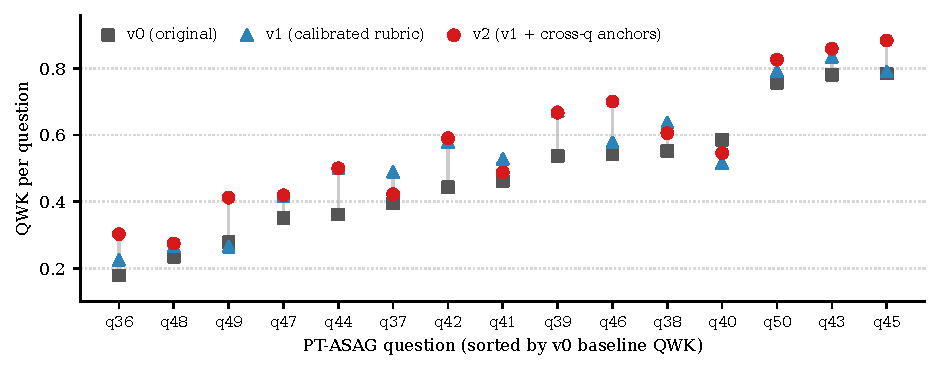
\includegraphics[width=0.92\textwidth]{herik_contrib/fig_rq1_per_question.pdf}
\caption{Per-question diagnosis QWK before (\textbf{v0}) and after calibration (\textbf{v1}, \textbf{v2}), ordered by \textbf{v0} QWK. \textbf{v2} improves over \textbf{v0} on $14$ of $15$ questions.}
\label{fig:rq1_per_q}
\end{figure*}

% Texto curto para Appendix -> Prompts (se desejar documentar o protocolo de H-02):
\paragraph{Diagnosis calibration prompts (\textbf{v1}/\textbf{v2}).} See \texttt{src/pln/prompts\_h02.py}. Variant \textbf{v1} constrains \texttt{conceitos} to expected keywords, clarifies independent teacher references, allows $0$--$3$ gaps, and separates omissions from conceptual errors. Variant \textbf{v2} prepends four median-length anchor responses (grades $0$--$3$) from question \texttt{q40} (or \texttt{q39} when evaluating \texttt{q40}), sampled deterministically from the $6{,}501$ unique PT-ASAG v2 answers outside \texttt{diag\_set} ($0$ overlap verified automatically).
